\documentclass{csnotes}

% ==============================================================================
% DOCUMENT SPECIFIC CUSTOMIZATIONS
% ==============================================================================

% --------------------------- START CUSTOMIZATIONS -----------------------------

% You can add any custom packages or commands specific to this document here

\usepackage{booktabs}

\setabstracttitle{Scopo del documento}

\newcommand{\whitepage}{
  \newpage
  \thispagestyle{empty}
  \mbox{}
  \newpage
}

% ---------------------------- END CUSTOMIZATIONS ------------------------------

% ==============================================================================
% DOCUMENT INFORMATION
% ==============================================================================
\title{Statistical Learning - Natural Language Processing}
\author{Riccardo Regina}
\date{\today}

% Additional information for the title page
\university{Università degli Studi Federico II di Napoli}
\department{Dipartimento d'Ingegneria Elettrica e Tecnologie dell'Informazione}
\course{Corso di Laurea Magistrale in Computer Science}
\subject{Statistical Learning}
\academicyear{Anno Accademico 2025/2026}

% ==============================================================================
% BIBLIOGRAPHY
% ==============================================================================
% Specify the .bib file with your bibliographic references
% Uncomment the following line when you have created the bibliography.bib file
\addbibresource{bibliography.bib}

% ==============================================================================
% INIZIO DOCUMENTO
% ==============================================================================

\begin{document}

\pagenumbering{gobble}

\maketitlepage{}
\whitepage{}

\begin{abstract}
  This document contains notes and study materials related to the \textit{Statistical Learning} course taught by Prof.~A.~Corazza at the University of Naples Federico II during the academic year 2025/26.

  In particular, these notes cover the concepts introduced in \textit{Natural Language Processing}, entirely drawn from Yoav Goldberg's book \cite{goldberg2017neural}.

  \textbf{These notes are intended to support students in their learning journey and provide a reference resource for the topics discussed during the course. However, they do not replace the official materials or the instructor's lectures in any way.}
  This document is created by students, for students, and may therefore contain errors or inaccuracies.

  \begin{flushright}
    \vspace{2cm}
    \textbf{The author:}\\
    \href{https://github.com/riccardoregina}{Riccardo Regina} \\
  \end{flushright}
\end{abstract}
\whitepage{}

\newgeometry{top=2cm}
\tableofcontents
\restoregeometry{}

\whitepage{}

\pagenumbering{arabic}
\setcounter{page}{1}

\chapter{Introduction to Natural Language Processing}

Natural Language Processing (NLP) is the field of study that focuses on the interaction between computers and human language. Its goal is to enable machines to understand, interpret, and generate human language in a way that is both meaningful and useful.

NLP is inherently interdisciplinary, drawing from linguistics, computer science, and artificial intelligence. It addresses the challenge of bridging the gap between the structured logic of machines and the complexity of human communication, which is rich in ambiguity, context, and cultural nuances.

The study of NLP is compelling because it allows us to automate and scale the understanding of vast amounts of textual data, from social media posts to scientific literature. By doing so, it unlocks new possibilities for extracting insights, improving accessibility, and creating more intuitive human-computer interfaces. NLP powers applications that we use daily, such as translation tools, virtual assistants, and sentiment analysis systems, making it a cornerstone of modern technology and a key driver of innovation in how we interact with information.
\chapter{Features}

\begin{observation}{Reference}
    Yoav Goldberg, Neural Network Methods for Natural Language Processing.
    Part II, Chapter 6.
\end{observation}

In language processing, feature vectors $\mathbf{x}$ are derived from textual data, in order to reflect various linguistic properties of the text. This process of derivation is called \textbf{feature extraction} and is done by a feature function $f$.

Deciding on the right features is a fundamental part of a successful machine learning project. \textbf{While deep learning alleviates a lot of the need for feature engineering, a set of core features still needs to be defined.}

\section{Types of Classification Problems in NLP}
In NLP, there are several types of classification problems, each depending on the type of input:

\begin{itemize}
    \item \textbf{Word}: We are faced with a word and need to determine something about it. This kind of problem is rare as words seldom appear in isolation.
    \item \textbf{Texts}: We are faced with a piece of text, such as a phrase, sentence, paragraph, or document, and must determine something about it. This is called \textbf{document classification}.
    \item \textbf{Paired Texts}: We are given a pair of words or longer texts and need to determine something about the relations between them.
    \item \textbf{Word in Context}: We are given a piece of text and a particular word (or phrase, letter, etc.), and need to determine something about the word in that context.
    \item \textbf{Relation Between Two Words}: We are given two words or phrases within a larger context and need to determine something about the relations between them.
\end{itemize}

\begin{quote}
    \textbf{Definition:} A \textbf{word} is the smallest unit of meaning, e.g., \textit{New York}, \textit{forgets}. In general, we distinguish between words and tokens. A \textbf{token} is the output of a tokenizer and can be a single word, multiple words, or part of a word. However, we will often use \textit{word} and \textit{token} as synonyms.
\end{quote}

\section{Features for NLP}
As words and letters are discrete items, features in NLP often take the form of indicators or counts. An \textbf{indicator feature} takes a value $0$ or $1$ depending on the existence of a condition (e.g., the word \textit{dog} is present). A \textbf{count} takes a value depending on the number of occurrences of some event (e.g., the word \textit{dog} appears 20 times in the document).

\subsection{Directly Observable Properties}
We list some properties that we can observe directly from the input, depending on the input type.

\subsubsection{Single Words}
When we only have a word, without any context, our main source of information is the letters comprising the word and their order, including things like prefixes, suffixes, capital letters, and numbers. We could also look at external sources of information to see how many times that word appears in collections of texts.

\begin{itemize}
    \item \textbf{Lemmas and Stems}: Given a single word or a word with a very limited context, we could look at its \textbf{lemma}, the dictionary entry (e.g., \textit{booking}, \textit{booked}, \textit{books} will all be reduced to \textit{book}). Lemmatization may not work well with misspelled words. A coarser process than lemmatization, which can work with any sequence of letters, is called \textbf{stemming}. Its product is not necessarily a valid word (e.g., \textit{picture}, \textit{pictures}, \textit{pictured} will all be reduced to the stem \textit{pictur}).

    \item \textbf{Lexical Resources}: An additional source of information is \textbf{lexical resources}, which are essentially dictionaries meant to be accessed programmatically. They map words to other words or descriptions, providing additional information (e.g., a word may be linked with all its possible meanings, declensions, synonyms, etc.). Examples include WordNet (1998), FrameNet (2004), VerbNet (2000), and The Paraphrase Database (2013). Lexical resources are not used in neural network approaches, but this may change.

    \item \textbf{Distributional Information}: To understand the meaning of a word, we may look at words that behave similarly, i.e., their distributions and typical contexts. This property is complex and will be discussed in depth later.
\end{itemize}

\subsubsection{Features for Text}
When dealing with a text, we typically count its words and look at their order.

\begin{itemize}
    \item \textbf{Bag of Words (BOW)}: We look at the histogram of words within the text, considering each word count as a feature.
    \item \textbf{Weighting}: We can integrate statistics based on external information, focusing on words that appear many times in the given text but few times in a set of external documents. This highlights words characteristic of the text. When using the bag-of-words approach, it is common to use TF-IDF.
\end{itemize}

\subsubsection{Features of Words in Context}
When considering a word within a sentence, phrase, or document, the directly observable features of the word are its position and the words or letters surrounding it. Words closer to the target tend to be more informative, but distant words may also influence the target (e.g., in Latin, verbs are typically at the end of a phrase, far from the subject).

\begin{itemize}
    \item \textbf{Windows}: It is common to focus on the immediate context of a word by considering a \textbf{window} surrounding it, i.e., $k$ words on each side, where typical values for $k$ are $2, 5, 10$. A window can be seen as a smaller bag of words. Since it is smaller, we may also consider the positions of words within it, which can provide useful information. We take the identity of words as features, e.g., for \textit{the brown fox \textbf{jumped} over the lazy dog}, the set of features is $\{w_{-2}=\text{brown}, w_{-1}=\text{fox}, w_{+1}=\text{over}, w_{+2}=\text{the}\}$.

    \item \textbf{Position}: Besides the context of the word, we may be interested in its absolute position within a sentence.
\end{itemize}

\subsubsection{Features for Word Relations}
When considering two words in context, besides their position and the words surrounding them, we can also look at the words between them and the distance between the two words.

\subsection{Inferred Properties}
Sentences in natural language have structures beyond the linear order of their words. This structure follows an intricate set of rules that are not directly observable. These rules are collectively referred to as \textbf{syntax}.

While the exact structure of language is still a mystery, a subset of phenomena governing language are well-documented and understood. Besides observable properties, we can look at inferred linguistic properties, such as:
\begin{itemize}
    \item The \textbf{part-of-speech (POS)} of a word within a text (e.g., noun, verb, adjective, determiner).
    \item The \textbf{syntactic role} of a word (e.g., subject, object of a verb, main verb).
    \item The \textbf{semantic role} of a word (e.g., in \textit{the key opened the door}, \textit{key} is an instrument, while in \textit{the uncle opened the door}, \textit{uncle} is an agent).
\end{itemize}

When considering two words in context, we can consider how close they are in the syntactic dependency tree of the sentence.

When moving beyond sentences, i.e., when studying relations between sentences rather than within them, we may want to understand whether the second sentence is an elaboration, contradiction, or effect of the first. Additionally, in natural language, we observe the phenomenon of \textbf{anaphora}. For example, in \textit{The boy opened the door with a key. He would have been happier if it was already open.}, \textit{He} refers to \textit{The boy}, while \textit{it} refers to \textit{the door}, not \textit{the key}.

Many deep learning experts argue that using manually crafted linguistic concepts is unnecessary, as neural networks can learn them on their own. However, some studies show that these concepts are still valuable in certain stages of a machine learning approach.

\subsection{Core vs. Combination Features}
In many cases, we are interested in a \textbf{conjunction of features} rather than individual ones. For example, the indicators \textit{the word `book' appeared in a window} and \textit{POS=verb appeared in a window} are useless alone but meaningful when combined. The combined indicator \textit{the word `book' with POS=verb appeared in a window} is much more informative about the meaning of the sentence.

However, linear models cannot assign a score to a conjunction of events that is not a sum of their individual scores unless the conjunction itself is modeled as its own feature. Thus, when designing features for a linear model, we must define not only the core features but also many combination features.

Neural networks do not suffer from this problem. If we use neural networks, we can specify only the core features and rely on the network's non-linearity. However, in some cases, neural networks do not surpass linear models with hand-crafted features.

\subsection{Ngrams}
A special case of feature combination is \textbf{ngrams}, consecutive word sequences of length $n$. A bag-of-bigrams representation is more powerful than bag-of-words because it can capture bigrams like \textit{New York} or \textit{not good}.

A priori, it is hard to know the optimal value for $n$. The common solution is to include all ngrams up to a given length and let the model's regularization discard the less interesting ones by assigning them very low weights.

However, a multi-layer perceptron (MLP) fed with a BOW input vector cannot infer ngram features on its own because a BOW vector does not provide positional information, and vanilla MLPs do not capture positional patterns.

To provide positional information, we can feed our MLP with an input vector that includes features like $w_{-2}=X$, $w_{-1}=Y$.

More specialized neural network architectures, such as \textbf{convolutional networks} and \textbf{recurrent networks}, are designed to find informative ngram features from sequences of words of varying lengths.

\subsection{Distributional Features}
Until now, our treatment of words has been as discrete and unrelated symbols: the words \textit{pizza}, \textit{burger}, and \textit{chair} are equally similar (and dissimilar) to each other. We achieved some generalization by considering POS, lemmas, stems, dictionaries, and lexical resources like WordNet, but these solutions are limited. They either provide very coarse-grained distinctions or rely on specific, manually compiled dictionaries.

Unless we have a specialized list of foods, we will not learn that \textit{pizza} is more similar to \textit{burger} than to \textit{chair}, and it will be even harder to learn that \textit{pizza} is more similar to \textit{burger} than to \textit{ice cream}.

The \textbf{distributional hypothesis of language} states that the meaning of a word can be inferred from the contexts in which it is used. By observing co-occurrence patterns of words across a large body of text, we can discover that the contexts in which \textit{burger} occurs are similar to those in which \textit{pizza} occurs, less similar to those in which \textit{ice cream} occurs, and very different from those in which \textit{chair} occurs.

Many algorithms have been developed over the years to leverage this property, learning generalizations of words based on their contexts. These can be broadly categorized into:
\begin{itemize}
    \item \textbf{Clustering-based methods}: Assign similar words to the same cluster and represent each word by its cluster membership.
    \item \textbf{Embedding-based methods}: Represent each word as a vector such that similar words (words with similar distributions) have similar vectors.
\end{itemize}

However, care must be taken when using word similarity information, as it can have unintended consequences. For example, in some applications, it is useful to treat \textit{London} and \textit{Berlin} as similar, while in others (e.g., booking a flight or translating a document), the distinction is crucial.
\chapter{Case Studies}

\begin{note}{Reference}
    Yoav Goldberg, Neural Network Methods for Natural Language Processing.\cite{goldberg2017neural}
    Part II, Chapter 7.
\end{note}

After discussing the different sources of information available for deriving features from natural language text, we will now explore examples of concrete NLP classification tasks, and suitable features for them.
Of course, modern language models may achieve very high performance on these tasks, but they may also be overkill. In this chapter, we will see features that are useful to build simpler yet very powerful models.
When talking about performance, we should always keep in mind the related costs: large language model are often huge and require very powerful runtimes.

\section{Document classification}
In this section, we discuss features that are suitable for document classification tasks.

\subsection{Language identification}
We are given a text and want to classify it into one of a fixed set of languages. Bag-of-letter-bigrams is a very strong feature representation for this task.

\begin{example}{}
    For language identification, the \qi{bag-of-letter-bigrams} representation captures statistical patterns of consecutive letter pairs. Consider two texts: \qi{The quick brown fox jumps over the lazy dog} (English) and \qi{La veloce volpe marrone salta sul pigro cane} (Italian).
    Extracting and counting letter bigrams (ignoring spaces and punctuation) yields distinct distributions: English texts often contain bigrams like \qi{th}, \qi{he}, or \qi{qu}, while Italian texts feature bigrams like \qi{il}, \qi{ve}, or \qi{ce}. These bigram counts serve as features for a classifier, enabling it to distinguish between languages based purely on statistical patterns.
\end{example}

\subsection{Topic classification}
We are given a text and need to classify it into one of a predefined set of topics. If we do not have many training examples, it may be a good idea to consider lemmas or stems rather than entire words. When using BOW, the TF-IDF encoding is very powerful. However, a learning algorithm is often capable of coming up with the weighting on its own.

\subsection{Authorship attribution}
In the authorship attribution task, we are given a text and need to infer the identity of its author from a fixed set of possible authors, or other characteristics of the author of the text, such as their gender, their age, or their native language.

The kind of information used to solve this task is very different from that of topic classification---the clues are subtle and involve stylistic properties of the text rather than content words. For this reason, we may want to adopt features that focus on the structure rather than the content. We can do so by considering POS and function words, namely words like \textit{on, of, before}, as well as pronouns to capture the author's style. A good approximation of function words is the top-300 most frequent words in a large corpus.

\begin{example}{}
For instance, consider the following sentences \qi{The cat sat on the mat.} and \qi{Upon the mat, the cat did sit.}
While both convey similar content, their stylistic differences—such as the use of \qi{on} vs. \qi{upon}, or the presence of the auxiliary \qi{did}—can serve as features. 
These features help distinguish authors based on their unique stylistic patterns rather than the topics they discuss.
\end{example}

\section{Word in context}


\subsection{POS tagging}
In the parts-of-speech tagging task, we are given a sentence and need to assign the correct part-of-speech to each word in the sentence. The POS tags belong to a predefined set; for this example, assume we will be using the tagset of the Universal Treebank Project (UTP, 2017), containing 17 tags: 
\begin{itemize}
    \item \qi{ADJ}: Adjective, describes a noun. Example: \qi{lazy} in \qi{the lazy dog}.
    \item \qi{ADP}: Adposition (preposition or postposition). Example: \qi{in} in \qi{in the house}.
    \item \qi{ADV}: Adverb, modifies a verb, adjective, or other adverb. Example: \qi{quickly} in \qi{She ran quickly.}
    \item \qi{AUX}: Auxiliary verb, helps express tense, mood, or voice. Example: \qi{is} in \qi{She is running.}
    \item \qi{CONJ}: Coordinating conjunction, connects words or phrases. Example: \qi{and} in \qi{cat and dog}.
    \item \qi{DET}: Determiner, introduces a noun. Example: \qi{the} in \qi{the cat}.
    \item \qi{INTJ}: Interjection, expresses emotion. Example: \qi{Oh!} in \qi{Oh! That's surprising.}
    \item \qi{NOUN}: Noun, names a person, place, or thing. Example: \qi{dog} in \qi{the dog barks}.
    \item \qi{NUM}: Numeral, represents a number. Example: \qi{three} in \qi{three cats}.
    \item \qi{PART}: Particle, often part of phrasal verbs or idioms. Example: \qi{up} in \qi{give up}.
    \item \qi{PRON}: Pronoun, replaces a noun. Example: \qi{she} in \qi{She is happy.}
    \item \qi{PROPN}: Proper noun, names a specific entity. Example: \qi{John} in \qi{John is here.}
    \item \qi{PUNCT}: Punctuation, marks the end of a sentence or separates clauses. Example: \qi{.} in \qi{Hello.}
    \item \qi{SCONJ}: Subordinating conjunction, introduces a dependent clause. Example: \qi{because} in \qi{She left because she was tired.}
    \item \qi{SYM}: Symbol, represents a non-linguistic symbol. Example: \qi{\$} in \qi{\$100}.
    \item \qi{VERB}: Verb, expresses an action or state. Example: \qi{run} in \qi{She runs fast.}
    \item \qi{X}: Other, for words that don't fit into the above categories. Example: \qi{abc} in \qi{the word abc}.
\end{itemize}

Part-of-speech tagging is usually modeled as a structured task---the tag of the first word may depend on the tag of the third one---but it can be approximated quite well by classifying each word in isolation into a POS-tag based on a window of two words to each side of the word. If we tag the words in a fixed order, for example from left to right, we can also condition each tagging prediction on tag predictions made on previous tags.

\begin{example}{}
    Consider the sentence:
    \qi{The lazy dog slept.}
    The corresponding POS tags using the UTP tagset are:
    \qi{DET ADJ NOUN VERB PUNCT}
\end{example}

However, we will see that bidirectional recurrent networks (biRNN) achieve better performance by considering both directions.

\subsection{Named entity recognition}
In the named-entity recognition (NER) task, we are given a document and need to find named entities such as Milan, John Smith, McCormik Industries, and Paris, as well as to categorize them into a predefined set of categories such as LOCATION, ORGANIZATION, PERSON, or OTHER.

\begin{note}{}
    Note that this task is context-dependent, as Milan can be a location (the city) or an organization (a sports team, \qi{Milan played against Barcelona Wednesday evening}), and Paris can be the name of a city or a person.
\end{note}{}

NER is usually modeled as a sequence tagging task like POS tagging. In particular, in NER, we use BIO-encoded tags: 
\begin{itemize}
    \item \qi{O}: Outside, not part of any named entity. Example: \qi{The} in \qi{The man lives in Rome.}
    \item \qi{B-PER}: Beginning of a person name. Example: \qi{John} in \qi{John Doe works here.}
    \item \qi{I-PER}: Inside (continuation) of a person name. Example: \qi{Doe} in \qi{John Doe works here.}
    \item \qi{B-LOC}: Beginning of a location name. Example: \qi{New} in \qi{New York is a city.}
    \item \qi{I-LOC}: Inside (continuation) of a location name. Example: \qi{York} in \qi{New York is a city.}
    \item \qi{B-ORG}: Beginning of an organization name. Example: \qi{Google} in \qi{Google LLC was founded in 1998.}
    \item \qi{I-ORG}: Inside (continuation) of an organization name. Example: \qi{LLC} in \qi{Google LLC was founded in 1998.}
    \item \qi{B-MISC}: Beginning of a miscellaneous entity. Example: \qi{Titan} in \qi{Titan is a moon of Saturn.}
    \item \qi{I-MISC}: Inside (continuation) of a miscellaneous entity. Example: \qi{Saturn} in \qi{Titan is a moon of Saturn.}
\end{itemize}

\begin{example}{}
    \qi{John Smith, president of McCormik Industries visited his niece Paris in Milan, reporters say.} should produce the output \qi{John/B-PER Smith/I-PER ,/O president/O of/O McCormik/B-ORG Industries/I-ORG visited/O his/O niece/O Paris/B-PER in/O Milan/B-LOC.}
\end{example}

So, given the analogies, the set of features for this task is quite similar to the POS tagging one.

\subsection{Preposition sense disambiguation}
Prepositions, words like \textit{on, in, with}, and \textit{for}, serve for connecting predicates with their arguments and nouns with their prepositional modifiers. Prepositions are very common and also very ambiguous. For example, consider the word \qi{for}: 
\begin{itemize}
    \item[a)] \qi{we went there for lunch}
    \item[b)] \qi{he paid for me}
    \item[c)] \qi{we ate for two hours}
    \item[d)] \qi{he would have left for home, but it started raining}
\end{itemize}

In (a), ``for'' indicates purpose, in (b) a beneficiary, in (c) a duration, and in (d) a location. 
In order to fully understand the meaning of a sentence, one should arguably know the correct senses of the prepositions within it. 
The preposition-sense disambiguation task deals with assigning the correct sense to a preposition in context, from a finite inventory of senses.

Linguists say that to understand a preposition, we must look at its verb (called governor) and its object. We could use some heuristics or a dependency parser or both.
For example, in (a), the governor is \qi{went} and the object \qi{lunch}, so the most likely meaning of \qi{for} is purpose.
Similarly, in (c), the governor is \qi{ate} and the object is \qi{hours}, suggesting that \qi{for} is indicating a duration.

\section{Relation between two words in context}
\subsection{Arc-factored parsing}
In the dependency parsing task, we are given a sentence and need to return a syntactic dependency tree over it. Each word is assigned a parent word, except for the main word of the sentence whose parent is a special \texttt{*ROOT*} symbol.

One approach to modeling the task is the arc-factored approach, where each of the possible $n^{2}$ word-word relations (arcs) is assigned a score independent of the others, and then we search for the valid tree with the maximal overall score. The score assignment is made by a trained scoring function \texttt{ARCSCORE($h$, $m$, sentence)}, receiving a sentence as well as the indices $h$ and $m$ of two words within it that are considered as candidates for attachment ($h$ is the index of the candidate head-word and $m$ is the index of the candidate modifier).

As features, we should use words and their POS tags. One could replace words with their embeddings. Another useful feature is the signed distance ($|h - m|$) between the head and the modifier.

\begin{example}{}
In the arc-factored parsing approach, we consider the sentence \qi{The cat chased the mouse.} and assign part-of-speech (POS) tags to each word:

\begin{center}
\begin{tabular}{c c c}
\hline
Index & Word & POS Tag \\
\hline
0 & The & DET \\
1 & cat & NOUN \\
2 & chased & VERB \\
3 & the & DET \\
4 & mouse & NOUN \\
5 & . & PUNCT \\
\end{tabular}
\end{center}

If we train correcly the scoring function, then the highest-scoring valid tree for this sentence should be:

\begin{center}
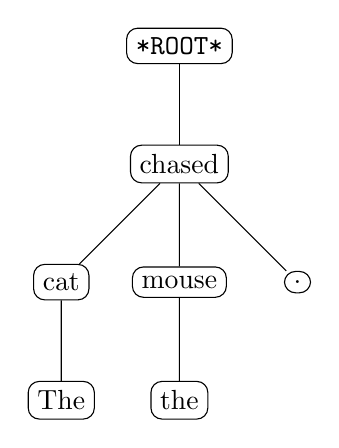
\begin{tikzpicture}[
    level distance=1.5cm,
    level 1/.style={sibling distance=3cm},
    level 2/.style={sibling distance=1.5cm},
    every node/.style={draw, rectangle, rounded corners, thin}
]
\node {\texttt{*ROOT*}}
    child { node {chased}
        child { node {cat}
            child { node {The} }
        }
        child { node {mouse}
            child { node {the} }
        }
        child { node {.} }
    };
\end{tikzpicture}
\end{center}
Note that, in standard dependency parsing, punctuation marks (like the final dot) are typically included in the dependency tree. They are usually attached to the head of the clause or sentence they terminate.
\end{example}
\chapter{Inputs}

\begin{observation}{Reference}
    Yoav Goldberg, Neural Network Methods for Natural Language Processing.
    Part II, Chapter 8.
\end{observation}

\section{Features Encoding for Neural Networks}

Features must be designed with the downstream task in mind, but once we have them, how should we encode them into an input to feed a network?

\section{One-hot encoding}
In linear models of the form
\( f(\mathbf{x}) = \langle \mathbf{x}, \mathbf{w} \rangle + \mathbf{b} \),
it is common to think in terms of indicator functions and assign a unique dimension for each possible feature.
For example, when considering a bag-of-words representation over a vocabulary of \( 40{,}000 \) items, \(\mathbf{x}\) will be a sparse vector with \( 40{,}000 \) components, where the non-null components represent the words contained in the input text.

\begin{quote}
    \textbf{Note:} Let's consider that \(\mathbf{x}\) contains a window of five words.
\end{quote}

If we want to give positional information, \(\mathbf{x}\) must be a concatenation of \(5\) input vectors, each with \(39{,}999\) zero-valued components and only one one-valued component, corresponding to the index of the word. This leads \(\mathbf{x}\) to be \(200{,}000\)-dimensional. In this way, the weight vector would also be \(200{,}000\)-dimensional.

In general, to represent a feature in a one-hot encoding fashion, we must create a vector of dimension \(d\), where every component is zero-valued except one, corresponding to the index of the feature value among the \(d\) possible values.

\section{Feature embeddings}
The biggest conceptual jump when moving from sparse-input linear models to deeper nonlinear models is to stop representing each feature as a unique dimension in a one-hot representation and instead represent them as \textbf{dense vectors}. That is, each core feature is embedded into a \(d\)-dimensional space and represented as a vector in that space. The dimension \(d\) is usually much smaller than the number of features. For example, each item in a vocabulary of \(40{,}000\) items can be represented as a \(100\) or \(200\)-dimensional vector rather than a \(40{,}000\)-dimensional one-hot encoded vector.

The embeddings are treated as parameters of the network and are trained like the other parameters of the function to learn. The general structure for an NLP classification system based on a feed-forward neural network is:
\begin{enumerate}
    \item Extract a set of core features \( f_{1}, \dots, f_{k} \) that are relevant for predicting the output class.
    \item For each feature \( f_{i} \), retrieve the corresponding vector \( v(f_{i}) \).
    \item Combine the vectors (either by concatenation, summation, or a combination of both) into an input vector \(\mathbf{x}\).
    \item Feed \(\mathbf{x}\) into a nonlinear classifier (feed-forward neural network).
\end{enumerate}

\section{A comparison}
One-hot encoded input vectors have very high dimensionality, and their components are independent, while input vectors built on embeddings have low dimensionality, and their components do have relations.

Besides that, the main benefit of embeddings is their \textbf{generalization power}: in a good set of embeddings (pre-trained embeddings, discussed later), similar words are near each other inside the dense space. Such good sets of embeddings can be obtained from a large corpus of text through algorithms that make use of the \textbf{distributional hypothesis}. Moreover, in a dense space, we can apply operations between the embeddings, so that:
\[
v(\text{king}) - v(\text{man}) + v(\text{woman}) \sim v(\text{queen}).
\]

However, in cases where we have a relatively few distinct features in the category and believe there are no correlations between the different features, we may use the one-hot representation.

\section{Combining dense vectors}
Each feature corresponds to a dense vector, and the different vectors need to be combined somehow. The prominent options are concatenation, summation (or averaging), and combinations of the two.

\subsection{Window-based features}
Consider the case of encoding a window of \(k\) words on the left and right side of a target word. Suppose \(k=2\), so \(a, b\) are on the left and \(c, d\) on the right. Suppose also that \(\mathbf{a}, \mathbf{b}, \mathbf{c}, \mathbf{d}\) are their vectors.

If we do not care about positional information, we can encode the window by summing \(\mathbf{a} + \mathbf{b} + \mathbf{c} + \mathbf{d}\). In this case, we could also calculate the average vector or a weighted sum like:
\[
\frac{1}{2}\mathbf{a} + \mathbf{b} + \mathbf{c} + \frac{1}{2}\mathbf{d}
\]
to give more importance to the words adjacent to the target. If we \textit{do} care, we can use concatenation, i.e., \([\mathbf{a}; \mathbf{b}; \mathbf{c}; \mathbf{d}]\). Finally, these encodings can be mixed.

\begin{note}{}
    When describing network layers that get concatenated vectors \(\mathbf{x}, \mathbf{y}, \mathbf{z}\) as input, some authors use explicit concatenation:
    \[
    [\mathbf{x}; \mathbf{y}; \mathbf{z}]\mathbf{W} + \mathbf{b},
    \]
    where \([\mathbf{x}; \mathbf{y}; \mathbf{z}]\) is a vector, while others use an affine transformation:
    \[
    \mathbf{x}\mathbf{U} + \mathbf{y}\mathbf{V} + \mathbf{z}\mathbf{W} + \mathbf{b}.
    \]
    If the weight matrices in the affine transformation are different from one another, the two notations are equivalent. By \textit{different}, we mean that the weights of one matrix are independent from the others, so an update of one matrix will not affect the others. In fact, in this case:
    \[
    \mathbf{W} = [\mathbf{W}; \mathbf{V}; \mathbf{U}].
    \]
\end{note}

\subsection{Variable number of features: continuous bag of words}
Feed-forward networks assume a fixed-dimensional input. However, in some cases, the number of features is not known in advance (e.g., in document classification, each word in the sentence may be a feature). We thus need to represent an unbounded number of features using a fixed-size vector. One way to achieve this is through a \textbf{continuous bag of words (CBOW)} representation: we average or weight-average the embeddings.

\section{Last but not least}
\subsection{Padding}
In some cases, your feature extractor will look for things that do not exist. For example, when working with parse trees, you may have a feature looking for the left-most dependent of a given word, but the word may not have any dependents to its left. Perhaps you are looking at the word two positions to the right of the current one, but you are at the end of the sequence, and two positions to the right is past the end.

What should be done in such situations? When using a bag-of-features approach (i.e., summing), you could leave the feature out of the sum. When using concatenation, you may provide a zero-vector in its place. These two approaches work fine technically but could be sub-optimal for your problem domain. Maybe knowing that there is no left-modifier is informative? The suggested solution is to add a special symbol (padding symbol) to your embedding vocabulary and use the associated padding vector in these cases. Depending on the problem, you may want to use different padding vectors for different situations (e.g., no-left-modifier may use a different vector than no-right-modifier). Such paddings are important for good prediction performance and are commonly used. Unfortunately, their use is not often reported or is quickly glossed over in many research papers.

\subsection{Unknown words}
Another case where a requested feature vector will not be available is for out-of-vocabulary (OOV) items. You are looking for the word on the left, observe the value \textit{variational}, but this word was not part of your training vocabulary, so you don’t have an embedding vector for it. This case is different from the padding case because the item is there, but you just don’t know it. The solution is similar: reserve a special symbol, \texttt{UNK}, representing an unknown token, for use in such cases. Again, you may or may not want to use different unknown symbols for different vocabularies. In any case, it is advised not to share the padding and the unknown vectors, as they reflect two very different conditions.

Instead of denoting all unknown words as \texttt{UNK}, we could use a more clever annotation that distinguishes very different words. For example, if the unknown word terminates with \textit{-ed}, we could assign it a \texttt{*ed} symbol; if it is a number, we could assign it \texttt{NUM}, etc. While there are ways to learn these symbols during training, this is often overkill, and it is simpler to handcraft them. This practice is often used but rarely mentioned in research papers.

What if, during training, the model never encounters an unknown word? In this case, if an unknown word appears during testing, we won't have an embedding for it. Hence, we need our model to handle the unknown word case. One of the best solutions is \textbf{word dropout}: at each iteration, each word will be dropped out with a predefined probability, i.e., replaced by \texttt{UNK} (or more fine-grained symbols). We should replace more frequently words that are less frequent, as these are more likely to be unknown. It would make no sense to prepare the model to face the event of not having an embedding for the word \textit{the}. There is no standard formula for dropout, but one could be:
\[
\frac{\alpha}{\alpha + \#w},
\]
where \(\#w\) is the frequency of the word \(w\) in the training set. Besides better adaptation to unknown words, word dropout may also be beneficial for preventing overfitting and improving robustness by not letting the model rely too much on any single word being present. When used this way, word dropout should be applied frequently, even to frequent words. However, when dropout is used like this, not all dropped words should be replaced as \texttt{UNK}, because this pattern is very unlikely to happen in test scenarios.

\subsection{Shared vectors}
Consider a case where you have a few features that share the same vocabulary. For example, when assigning a part-of-speech to a given word, the input has some features like the previous and the next word. Suppose these two are the same word. Should we share the two representative vectors? If we believe that these words may have slightly different meanings in different positions, then the answer is no. Otherwise, we could save memory, but this is true empiricism.

\subsection{Dimensionality}
How big should an embedding be? In current research (2017), the dimensionality of word-embedding vectors ranges between about 50 to a few hundred, and in some extreme cases, thousands. Since the dimensionality of the vectors has a direct effect on memory requirements and processing time, a good rule of thumb is to experiment with a few different sizes and choose a good trade-off between speed and task accuracy.

\subsection{Finite vocabulary}
What does it mean to associate an embedding vector for every word? Clearly, we cannot associate one with all possible values and need to restrict ourselves to every value from a finite vocabulary. This vocabulary is usually based on the training set or, if we use pre-trained embeddings, on the training set on which the pre-trained embeddings were trained. It is recommended that the vocabulary also include a designated \texttt{UNK} symbol, associating a special vector to all words that are not in the vocabulary.
\chapter{Language Modeling}

\begin{observation}{Reference}
    Yoav Goldberg, Neural Network Methods for Natural Language Processing.
    Part II, Chapter 9.
\end{observation}

Language modeling is the task of assigning a probability to sentences in a language. Besides that, the language models also assign a probability to a given word (or sequence of words) to follow a sequence of words.

\begin{example}{}
A language model answers to questions like:
\begin{enumerate}
    \item what is the probability of seeing the word 'barking' after 'the dog is'?
    \item what is the probability of seeing the sentence 'the dog is barking'?
\end{enumerate}
As we will see in a moment, these two questions require the same quantity of information.
\end{example}

Formally, given a sequence of words $w_{1:n}$, we want to estimate $\Pr(w_{1:n})$, that is
$$
\Pr(w_{1:n}) = \Pr(w_{1})\Pr(w_{2}|w_{1})\dots \Pr(w_{n}|w_{1:n-1})
$$

\begin{observation}{Note}
Note that calculating $\Pr(w_{n}|w_{1:n-1})$ is as complex as calculating $\Pr(w_{1:n})$. In fact, according to the definition of conditioned probability,
$$
\Pr(w_{n}|w_{1:n-1}) = \frac{\Pr(w_{n})}{\Pr(w_{1:n})}
$$
In words, calculating the likelihood of the last word given the preceding ones is not easier than calculating the likelihood of the entire sentence.
\end{observation}

For this reason, many language models in the past make use of the $k$-th order Markov assumption, that is
$$
\Pr(w_{i}|w_{1:i-1}) = \Pr(w_{i}|w_{i-k:i-1})
$$
At this point, the probability of the sentence becomes
$$
\Pr(w_{1:n}) = \prod_{i=1}^{n}\Pr(w_{i}|w_{i-k:i-1})
$$
with $\set{w_{-k}, w_{-k+1},\dots, w_{0}}$ being special padding symbols. Our task is then to accurately estimate $\Pr(w_{i+1}|w_{i})$ given large amounts of text.

\section{Perplexity}
Even though language models are typically evaluated on the downstream task, there is an intrinsic metric called \textbf{perplexity} that indicates how much the language model is confident on sequences of a given corpus. Let $LM$ be the language model and a text corpus of $n$ words, then perplexity is defined as:
$$
2^{-\frac{1}{n}\sum_{i=1}^{n}\log LM(w_{i}|w_{1:i-1})}
$$
Good language models will have a low score of perplexity.

\begin{observation}{Note}
Perplexities are corpus-specific. If you want to compare two LMs, you must do it on the same corpus.
\end{observation}

\section{Traditional models}
The traditional LM approach assumes a $k$-th order Markov assumption and tries to find good estimates $\hat{p}(w_{i+1}=m|w_{i-k:i})$. Let $\#(w_{i:j})$ be the count of the sequence $w_{i:j}$ inside the text corpus. It can be proven that the maximum likelihood estimate (MLE) of $\hat{p}(w_{i+1}=m|w_{i-k:i})$ is
$$
\hat{p}_{\text{MLE}}(w_{i+1}=m|w_{i-k:i}) = \frac{\#(w_{i-k:i+1})}{\#(w_{i-k:i})}
$$
A big downside of this approach is that if any sequence $w_{i-k:i+1}$ is never encountered in the corpus (i.e., its count is zero), then the estimate is zero on the entire corpus (since the probability of a sentence is calculated via the chain rule), and the perplexity is infinite. To avoid this, we can use smoothing techniques that ensure a non-null probability for every single sequence or else use a totally different approach like neural models.

\section{Neural models}
A simple model was presented by Bengio (2003) and is based on a feed-forward neural network. The network is fed with a $k$-gram, representing a context window, $\mathbf{x} = (v(w_{1}); v(w_{2}) \dots; v(w_{k}))$, where $v(w_{i})$ is the embedding of word $w_{i}$, and outputs a probability distribution $\mathbf{y}$ over the entire vocabulary $V$.

The distribution vector $\mathbf{y}$ is obtained by applying a softmax layer. The component $y_{i}$ of maximum value will represent the next most probable word. The vocabulary $V$ also contains special symbols like \texttt{UNK}, \texttt{<s>} (start symbol), \texttt{</s>} (end symbol).

\textbf{The training is unsupervised} (actually, automatically supervised) since the dataset contains all $k$-grams whose target is the subsequent word. The loss function is cross-entropy.

Concerning performance and complexity, enlarging the window from $k$ to $k+l$ is linear in the number of parameters, which is a modest increase compared to the polynomial increase in traditional, count-based models. However, the biggest limitation is the cost of the softmax layer, which for large vocabularies can be prohibitive. A good review and comparison of the techniques that try to solve this limitation is available in Chen et al. (2016, \url{http://aclweb.org/anthology/P16-1186}).

Putting aside the prohibitive cost of using the large output vocabulary, the model has very appealing properties. It achieves better perplexities than state-of-the-art traditional language models such as Kneser-Ney smoothed models and can scale to much larger orders.

\section{Using language models for generation}
Once we have trained a language model, we can generate new sentences by letting it predict the next words. Note that picking the most probable word at each step might result in a globally less probable sentence, while using \textbf{beam search} might lead to a more probable one.

\begin{observation}{Beam search}
Instead of only keeping the single best candidate (greedy search) or all possible candidates (exhaustive search) at each step, beam search keeps track of the top-$k$ most probable partial sequences (called hypotheses) at each step. Start with an empty sequence (or a start token, e.g., \texttt{<s>}). At each step:
\begin{enumerate}
    \item For each of the $k$ best partial sequences, generate new sequences by appending each possible next word and calculate the score.
    \item Keep only the top-$k$ sequences with the highest scores.
    \item Repeat until a stopping condition is met (e.g., reaching a maximum length or generating an end token, e.g., \texttt{</s>}).
\end{enumerate}
Finally, return the highest-scoring complete sequence from the remaining candidates.
\end{observation}
\chapter{Pre-trained Word Representation}

In this chapter, we will see how to construct word embeddings.

\begin{note}{Reference}
    Yoav Goldberg, Neural Network Methods for Natural Language Processing.\cite{goldberg2017neural}
    Part II, Chapter 10 and 11.
\end{note}
If we are interested in task A, for which we have only a very limited amount of labeled data, but there is an auxiliary task B for which we have much more labeled data, we may want to pre-train our word embeddings on task B and then use them for training task A.

The common case is that we do not have an auxiliary task with large enough amounts of annotated data (or maybe we want to help bootstrap the auxiliary task training with better vectors). In such cases, we resort to \textbf{self-supervised} auxiliary tasks, which can be trained on huge amounts of unannotated text.

All the algorithms to find word embeddings are based on the \textit{distributional hypothesis}.

\section{Word-context Matrices}
A word-context matrix $\mathbf{M}$ combines all words with all possible contexts. Each row $i$ represents a word, each column $j$ represents a context in which words can occur, and a matrix entry $\mathbf{M}_{i,j}$ quantifies the strength of association between a word and a context in a large corpus.

In this way, each word is represented as a sparse vector in high-dimensional space, encoding the weighted bag of contexts in which it occurs. Different definitions of contexts and different ways of measuring the association between a word and a context give rise to different word representations.

Formally, each entry of $\mathbf{M}$ is defined as $\mathbf{M}_{i,j}^{f}=f(w_{i},c_{j})$, where $f$ is an association measure of the strength between the word $w_{i}\in V_{W}$ and the context $c_{j} \in V_{C}$, where $V_{W}$ and $V_{C}$ are, respectively, the set of words and the set of contexts.

\textbf{There are two main approaches to construct embeddings: the distributional approach and the distributed one.} 
The first is based on frequencies, while the second involves training a neural network. Even though they may be different at first glance, they are equivalent, i.e., they give interchangeable outputs.

\section{Similarity measures}
Different distance functions can be used to measure the distances between word vectors, which are taken to represent the semantic distances between the associated words. A common and effective measure is the \textbf{cosine similarity}, which measures the angle between two vectors:
\[
\text{sim}_{\cos}(u,v)=\frac{u\cdot v}{\| u \|_{2}\cdot \| v \|_{2}}
\]
Another popular measure is the \textbf{generalized Jaccard similarity}, defined as:
\[
\text{sim}_{\text{Jaccard}}(u,v)=\frac{\sum_{i}\min(u_{i}, v_{i})}{\sum_{i}\max(u_{i}, v_{i})}
\]

\section{Distributional approach: Word-context weighting}
The function $f$ is usually based on counts from a large text corpus. Let $\#(w,c)$ be the occurrences of the word $w$ in the context $c$ in the corpus $D$, and let
\[
|D|=\sum_{\substack{w\in V_{W}\\c\in V_{C}}}\#(w,c)
\]
be the corpus size.

At first, one could think to define $f(w,c)$ to be $f(w,c)=\#(w,c)$ or a normalized version $f(w,c)=\frac{\#(w,c)}{|D|}$. However, this definition has the side effect of assigning high weights to word-context pairs involving very common contexts. For example, assuming the context is the preceding word, \textit{cat} will frequently appear in contexts \textit{the cat} and \textit{a cat}. However, \textit{the} and \textit{a} are not informative at all since they appear with almost every word.

To solve this, we have to assign higher weights to a word-context pair involving a context that co-occurs more with the given word than with other words.

\begin{note}{}
This kind of approach is very similar to the one used in TF-IDF.
\end{note}

An effective metric that captures this behavior is the \textbf{pointwise mutual information} (PMI):
\[
\text{PMI}(w,c)=\log\frac{\Pr(w,c)}{\Pr(w)\Pr(c)}
\]
where the probabilities can be calculated as frequencies. However, for $\Pr(w,c)=\#(w,c)=0$, we observe $\text{PMI}(w,c)=-\infty$. To avoid this, we can use \textbf{positive PMI}, which is defined as:
\[
\text{PPMI}(w,c)=\max\{0, \text{PMI}(w,c)\}
\]

This function has a side effect: it assigns high values to rare events. For example, if two words occur only once but in the same context, they will receive a high $\text{PMI}$. To overcome this, one should apply a count threshold before using the $\text{PMI}$ metric.

A potential obstacle to representing words as the explicit set of contexts in which they appear is that of data sparsity and high dimensionality. The former can lead to incorrect values of $f(w,c)$ because we did not observe enough data points, while the latter can lead to performance issues.

To alleviate both problems, we can perform a dimensionality reduction technique such as the \textbf{singular value decomposition} (SVD), which factorizes the matrix $\mathbf{M}$ into two narrow matrices $\mathbf{W}\in \mathbb{R}^{|V_{W}|\times d}$, the word matrix, and $\mathbf{C}\in \mathbb{R}^{|V_{C}|\times d}$, the context matrix, such that $\mathbf{W}\mathbf{C}^{T}=\mathbf{M}'$ where $\mathbf{M}'$ is the matrix with $\text{rank}(\mathbf{M}')=d$ that is closer, in terms of $L_{2}$, to $\mathbf{M}$.

We can see $\mathbf{M}'$ as a smoothed version of $\mathbf{M}$: based on robust patterns in the data, some of the measurements are ``fixed,'' e.g., words are added to contexts that they were not seen with if other words in this context seem to co-locate with each other.

Moreover, the matrix $\mathbf{W}$ allows us to represent each word as a dense $d$-dimensional vector, where $d \ll |V_{C}|$ (typical values are $50 < d < 300$). As we already said, this allows generalization: operations between word vectors will preserve semantic meaning.

\section{Distributed representations}
Unlike distributional representations, in which each dimension corresponds to a specific context the word occurs in (unless SVD is applied), the dimensions in the distributed representation are not interpretable, and specific dimensions do not necessarily correspond to specific concepts.

The distributed nature of the representation means that a given aspect of meaning may be captured by (distributed over) a combination of many dimensions, and that a given dimension may contribute to capturing several aspects of meaning.

Note that these characteristics are equally achieved by applying SVD to a distributional representation.

\section{Collobert and Weston}
A neural network for language modeling must output a distribution of words given the context. This requires a softmax layer, whose cost may be prohibitive for large vocabularies.

Collobert and Weston relaxed the probabilistic output constraint so that the model only attempts to assign a score to each word.

Another constraint for language modeling is that we must be able to apply the chain rule on the context to calculate a sentence-level probability. Collobert and Weston relaxed even this constraint by replacing the preceding $k$-gram context with a word window surrounding the target, that is, the model has to compute $\Pr(w_{3}|w_{1}w_{2}\square w_{4}w_{5})$ instead of $\Pr(w_{5}|w_{1}w_{2}w_{3}w_{4}\square)$.

The network is fed with an input vector $\mathbf{x}=(v_{c}(c_{1});\dots;v_{c}(c_{k});v_{w}(w))$, where $v_{c}$ and $v_{w}$ are, respectively, the context embedding function and the word embedding function. Both functions map a word to a $d_{emb}$-dimensional vector.

Then, the output score is calculated:
\[
\begin{aligned}
s(w, c_{1:k})&=z \\
z&=\mathbf{y} \cdot \mathbf{v} \\
\mathbf{y}&=g(\mathbf{x}\mathbf{U})
\end{aligned}
\]
where \(\mathbf{U}\) is the weight matrix of the hidden layer and \(\mathbf{v}\) is the global scoring vector, also a vector of weights.

The network is trained with a margin-based loss to score correct word-context pairs $(w, c_{1:k})$ over incorrect ones $(w', c_{1:k})$ with a margin of at least $1$. The loss is defined as:
\[
L(w, c_{1:k}, w')=\max\{0, 1 - (s(w,c_{1:k}) - s(w', c_{1:k}))\}
\]
where $w'$ is a random word sampled from the vocabulary: at each step, the training algorithm selects a word-context pair $(w, c_{1:k})$, samples a random $w'$, calculates the loss, and updates the weights $\mathbf{U}$, $\mathbf{v}$, and the word and context embeddings to minimize the loss.

When \(s(w,c_{1:k}) - s(w', c_{1:k}) \geq 1\), the loss is \(0\) and so the model is correctly assigning a high score to the correct pair and a low one to the wrong one.
On the other hand, when \(s(w,c_{1:k}) - s(w', c_{1:k}) < 1\), the loss is positive because the model is assigning similar scores to both the correct and incorrect pairs.

By maximizing the margin between different couples, we enforce the distributional law (words with similar contexts will have similar embeddings) while avoiding calculating softmax on huge embedding sets.

\section{Word2Vec}
Other word-embedding algorithms are CBOW and Skip-Gram, presented by Mikolov et al. in the Word2Vec suite.

Word2Vec replaces the margin-based ranking objective with a probabilistic one. Consider a set $D$ of correct word-context pairs and a set $\bar{D}$ of incorrect word-context pairs. The goal of the algorithm is to estimate the probability $\Pr(D=1|w,c)$, that is, the probability of assigning the pair $(w,c)$ to $D$.

This probability is defined as:
\[
\Pr(D=1|w,c)=\frac{1}{1 + e^{-s(w,c)}}
\]
and a probability constraint is added: $\Pr(D=1|w,c)=1-\Pr(D=0|w,c)$.

The corpus-wide objective of the algorithm is to maximize the log-likelihood of the data $D\cup \bar{D}$:
\[
\mathcal{L}(\Theta, D, \bar{D})=\sum_{(w,c) \in D}\log\Pr(D=1|w,c) + \sum_{(w,c) \in \bar{D}}\log\Pr(D=0|w,c)
\]
For each positive word $w\in D|_{w}$, sampled from the corpus, the training algorithm samples $k$ negative examples from the corpus $w_{1:k}$ and adds them to $\bar{D}|_{w}$, where $k$ is a hyperparameter. The negative words are sampled according to their frequency or smoothed versions of this criterion.

\subsection{CBOW}
The Continuous Bag Of Words (CBOW) variant of Word2Vec adds up the context vectors $c_{1:k}$ to a single aggregated context vector $c$:
\[
c=\sum_{i=1}^{k}c_{i}
\]
and simplifies the scoring function of Collobert and Weston:
\[
s(w,c)=w\cdot c
\]
so that we have:
\[
\Pr(D=1|w,c)=\frac{1}{1+e^{-(w\cdot c)}}
\]

\begin{note}{}
    This method is called CBOW because it adds up the context word embeddings into a single context vector, as one would do with BOW sparse vectors. Since we are instead working with continuous dense embedding vectors, this method is called Continuous BOW.
\end{note}

This variant decouples the context words from their positions: adding the context vectors discards positional information.

\subsection{Skip-gram}
The Skip-Gram variant decouples the context words even more: the $k$ context words are assumed independent, and each context word is treated as a stand-alone context. The probability is calculated as in the CBOW approach:
\[
\Pr(D=1|w,c)=\prod_{i=1}^{k}\Pr(D=1|w,c_{i})=\prod_{i=1}^{k} \frac{1}{1+e^{-(w\cdot c_{i})}}
\]
While this variant may seem too simple, it is very effective and commonly used.

\section{Limitations of distributional methods}
The distributional hypothesis leads to very interesting results but comes with some limitations:
\begin{itemize}
    \item \textbf{Lack of control on similarities}. Similarity between words can be of several types: consider the words \textit{cat}, \textit{dog}, \textit{tiger}. On the one hand, \textit{cat} is more similar to \textit{dog} than to \textit{tiger} because they are both pets, but, on the other hand, \textit{cat} is more similar to \textit{tiger} since they are both felines. The distributional methods provide very little control over the kind of similarities they induce. This could be controlled to some extent by the choice of conditioning contexts.
    \item \textbf{Antonyms}. Words that are the opposite of each other (antonyms) tend to appear in the same context. For example, something that is \textit{cold} may also be \textit{hot}. A distributional method may represent antonyms as very similar vectors.
\end{itemize}

\section{Word embeddings outside neural networks}
Besides neural networks, word embeddings can be used for several useful tasks, all of them based on word similarity:
\begin{itemize}
    \item \textbf{$k$-most-similar words}. Once we have embeddings (say) in a matrix $\mathbf{E}$ such that $\mathbf{E}_{i}=\mathbf{w}_{i}$ is the embedding of the $i$-th word, we can calculate a vector of similarities $\mathbf{s}=\mathbf{E}\mathbf{w}^{T}_{i}$ which tells us how much the vector \(\mathbf{w}_{i}\) is similar to all the other ones.
    \item \textbf{Word clustering}. Having word embeddings allows us to apply clustering algorithms and hence relate similar concepts.
    \item \textbf{Extend a group}. Say we have a group of words that we want to extend (e.g., a group of first names). We can calculate the average word embedding between them and take the $k$-most-similar words to extend the group.
    \item \textbf{Odd one out}. Similarly, say we have a group of words and want to find the one that does not belong to it. We can once again calculate the average word embedding and discard the most distant word embedding of the group.
    \item \textbf{Word analogies}. As already mentioned, word embeddings allow us to elegantly solve word analogies, e.g., \textit{Paris:France=X:Italy}, with simple linear algebra, that is $\mathbf{w}_{\text{Paris}}-\mathbf{w}_{\text{France}}+\mathbf{w}_{\text{Italy}}\sim \mathbf{w}_{\text{Rome}}$.
\end{itemize}

\begin{note}{}
    We are assuming that the word similarity is calculated as cosine similarity between the word embeddings.
\end{note}
\chapter{Recurrent Neural Networks}

\begin{observation}{Reference}
    Yoav Goldberg, Neural Network Methods for Natural Language Processing.
    Part III, Chapters 13-17.
\end{observation}

The main problem of vanilla feed-forward neural networks is that they do not consider hierarchical patterns and positions, instead treating each input component as independent. Moreover, these networks allow only a fixed size for the input, not allowing a variable length. Convolutional Neural Networks (CNNs) capture word order of the context, yet limited to local patterns and hence does not relate words that are far apart in the input sequence. CNNs also allow a fixed size input. Recurrent Neural Networks (RNNs) allow representing arbitrarily sized sequential inputs in fixed-size vectors, while capturing structural patterns in the input.

We will see RNNs as an abstraction: an interface for translating a sequence of inputs into a fixed sized output, that can then be plugged as components in larger networks.

\begin{note}{CNNs}
    Convolutional networks have been discussed in detail in another course. Here, we give just a note about naming. Since CNNs did arise from the computer vision setting, its concepts are recall images rather than linear sequences like text. However, these concepts can be well ported from 2D to 1D. For example, while it is common knowledge that images are made up of three channels (RGB), it can be not obvious for text. However, text can absolutely have different channels, such as the sequence of words, the sequence of the relative POS tags etc.
\end{note}

\section{The RNN abstraction}
Let $\mathbf{x}_{i:j}$ be the sequence of vectors $\mathbf{x}_{i},\dots,\mathbf{x}_{j} \in \mathbb{R}^{d_{in}}$. A RNN takes an input sequence $\mathbf{x}_{1:n}$ and returns a single output vector $\mathbf{y}_{n}\in \mathbb{R}^{d_{out}}$:
\[
\mathbf{y}_{n}=\text{RNN}(\mathbf{x}_{1:n})
\]
This implicitly defines an output vector $\mathbf{y}_{i}$ for each subsequence $\mathbf{x}_{1:i}$. We denote with $\text{RNN}^{*}$ the function returning the sequence of output vectors $\mathbf{y}_{1:n}$:
\[
\begin{aligned}
\mathbf{y}_{1:n}&=\text{RNN}^{*}(\mathbf{x}_{1:n}) \\
\mathbf{y}_{i}&=\text{RNN}(\mathbf{x}_{1:i})
\end{aligned}
\]
Then, the output vector $\mathbf{y}_{n}$ is used for further prediction. In fact, both CNNs and RNNs are used for feature extraction.

The RNN function provides a framework for conditioning on the entire history $\mathbf{x}_{1:n}$ without the need of the Markov assumption, which is typical of traditional language models. In fact, RNN-based language models result in very good perplexity scores.

More precisely, at each step, the RNN takes a new input vector $\mathbf{x}_{i}$ and a state vector $\mathbf{s}_{i-1}$, that contains information about the result of the previous step, and returns a new state vector $\mathbf{s}_{i}$ by means of a function $R$. Then, the state vector $\mathbf{s}_{i}$ is mapped to an output vector $\mathbf{y}_{i}$ using a simple deterministic function $O$.

When building a RNN, as one would do with a feed-forward network, one has to specify the input dimension $d_{in}$, the output dimension $d_{out}$. The state dimension, instead, is a function of $d_{out}$ i.e. $f(d_{out})$. So, a RNN is defined in detail as:
\[
\begin{aligned}
\text{RNN}^{*}(\mathbf{x}_{1:n};\mathbf{s}_{0})&=\mathbf{y}_{1:n} \\
\mathbf{y}_{i}&=O(\mathbf{s}_{i}) \\
\mathbf{s}_{i}&=R(\mathbf{s}_{i-1};\mathbf{x}_{i})
\end{aligned}
\]
with $\mathbf{x}_{i}\in \mathbb{R}^{d_{in}}$, $\mathbf{y}_{i} \in \mathbb{R}^{d_{out}}$, $\mathbf{s}_{i}\in \mathbb{R}^{f(d_{out})}$. Note that the functions $O$, $R$ are fixed but their behavior is modified through the network parameters $\theta$, which are updated during training.

Talking about training, it is important to say that RNNs are always placed inside a larger network and serve as a feature extractor. For this reason, the loss function depends on the downstream task. The only concern about training is hence how to build the computational graph of a RNN. This is fairly simple though: for finite input sequences, we can unroll the recursion into a computational sequence.

\section{Common RNN usage patterns}
As we already said, RNNs are used as feature extractors inside larger networks. Now, we will see the common patterns that are followed to integrate a RNN inside a more complex network.

\subsection{Acceptor}
One option is to use only the last output vector $\mathbf{y}_{n}$ as a pattern signal. This is a simple yet powerful use of RNNs since $\mathbf{y}_{n}$ depends on the entire input sequence $\mathbf{x}_{1:n}$.

\begin{example}{}
For example, this pattern can be used for POS-tagging, next-word prediction etc.
\end{example}

\subsection{Encoder}
Another way of using a RNN is to consider the output $\mathbf{y}_{n}$ as an encoding of the entire sequence $\mathbf{x}_{1:n}$. This encoding is then used as additional information together with other signals.

\subsection{Transducer}
We can treat the RNN as a transducer, producing an output $\mathbf{y}_{i}=\hat{\mathbf{t}}_{i}$ for each input $\mathbf{x}_{i}$ it reads in. In this way, we can compute a local loss signal $L_{\text{local}}(\hat{\mathbf{t}}_{i}, \mathbf{t}_{i})$ for each of the outputs $\hat{\mathbf{t}}_{i}$ based on a true label $\mathbf{t}_{i}$. The loss for the unrolled sequence will then be
\[
L(\hat{\mathbf{t}}_{1:n}, \mathbf{t}_{1:n})=\sum_{i=1}^{n}L_{\text{local}}(\hat{\mathbf{t}}_{i}, \mathbf{t}_{i})
\]
or using another combination of the local losses such as average or weighted average.

A very natural use-case of the transduction setup is for language modeling, in which a sequence of words $\mathbf{x}_{1:i}$ is used to predict a distribution over the $(i+1)$-th word. RNN-based language models provide vastly better perplexities than traditional language models, as already mentioned.

\section{Bi-directional RNNs (biRNNs)}
A RNN allows to condition the word $\mathbf{x}_{i}$ on the entire preceding word sequence $\mathbf{x}_{1:i-1}$. However, we have seen that also the following words $\mathbf{x}_{i+1:n}$ can be useful for prediction.

To do this, we use two RNNs: a forward RNN and a backward one. The forward $\text{RNN}(R^f, O^f)$ is fed with the word sequence $\mathbf{x}_{1:n}$ while the backward $\text{RNN}(R^b, O^b)$ with the reversed sequence $\mathbf{x}_{n:1}$. The two RNNs maintain, respectively, a forward state $\mathbf{s}^f_{i}$ and a backward state $\mathbf{s}^{b}_{i}$.
At each step, the two RNNs calculate, respectively, $\mathbf{y}^f_{i}=O^f(\mathbf{s}^f_{i})$ and $\mathbf{y}^b_{i}=O^b(\mathbf{s}^b_{i})$. The output of the $\text{biRNN}$ is the concatenation of the two output vectors. So,
\[
\begin{aligned}
\mathbf{y}_{i}&=[\mathbf{y}^f_{i};\mathbf{y}^b_{i}] \\
\mathbf{y}^f_{i}=O^f&(\mathbf{s}^f_{i}),\:\mathbf{y}^b_{i}=O^b(\mathbf{s}^b_{i}) \\
\mathbf{s}_{i}^f=R^f(\mathbf{s}^f_{i-1};\mathbf{x}_{i}&),\:\mathbf{s}_{i}^b=R^b(\mathbf{s}^b_{i-1};\mathbf{x}_{n+1-i})
\end{aligned}
\]

\section{Multi-layer (stacked) RNNs}
Since a RNN is a feature extractor, we can stack $k$ RNNs to extract "more features".

\begin{note}
While it is not theoretically clear what is the additional power gained by the deeper architecture of stacked RNNs, it was observed empirically that they work better than shallower ones on some tasks.
\end{note}

In a multi-layer RNN, $k$ RNNs are stack one on top of another so that the first RNN will take as input the sequence $\mathbf{x}_{1:n}$, the second RNN will take as input the output sequence of the first RNN and so on.

\begin{observation}{}
biRNNs can be stacked in a similar fashion.
\end{observation}

\section{RNN implementations}
We have previously described formally what a RNN is, but have not provided any implementation of the two functions $R$, $O$, which we are going to do now.

\subsection{Simple-RNN (S-RNN)}
Presented by Elman (1990) and then further explored by Mikolov (2012), the S-RNN is implemented as:
\[
\begin{aligned}
\mathbf{s}_{i}&=R(\mathbf{s}_{i-1};\mathbf{x}_{i})=g([\mathbf{s}_{i-1};\mathbf{x}_{i}]\cdot \mathbf{W} + \mathbf{b}) \\
\mathbf{y}_{i}&=O(\mathbf{s}_{i})=\mathbf{s}_{i}
\end{aligned}
\]
where $\mathbf{W}$ and $\mathbf{b}$ are learnable parameters.

Another variant, introduced by Jordan, makes $\mathbf{s}_{i}$ dependent directly on the preceding output $\mathbf{y}_{i-1}$ rather than $\mathbf{s}_{i-1}$.

\subsection{Gated architectures}
S-RNNs are difficult to train because of vanishing gradients: early input signals do not reach the final output because of the chain of products between $\mathbf{x}_{i}$ and $\mathbf{W}$. This is both a numerical limitation and a functional limitation: null gradients make it difficult to minimize the loss function and early signals that get lost in the process limit the conditioning window of the model.

To avoid this, we must find a way to preserve early input signals that are crucial. At the moment, the state vector $\mathbf{s}_{i}$ gets overwritten, without control, during the compute of $\mathbf{s}_{i+1}=R(\mathbf{s}_{i};\mathbf{x}_{i+1})$. We must therefore control this state update.

We can achieve this by introducing an access gate vector $\mathbf{g}\in\{0,1\}^{d_{in}}$ s.t. $R$ can only modify the state vector components $s_{j}$ s.t. $g_{j}=1$. We can implement this with a simple element-wise multiplication, also called hadamard-product:
\[
\mathbf{s}_{i+1}=\mathbf{x}_{i+1}\odot\mathbf{g} + \mathbf{s}_{i}\odot (1-\mathbf{g})
\]
Moreover, we want these gates to be learnable and so this calculation differentiable to allow gradient descent. We can then relax the hard gate constraint by allowing any real value and then apply a sigmoid function to force the value to be inside between $0$ and $1$, i.e. $\mathbf{g}\in (0,1)^{d_{in}}$.

\subsection{LSTM}
The Long Short-Term Memory (LSTM) architecture splits the state vector into two halves, where one half is treated as "memory cells" and the other as working memory. The memory cells are designed to preserve the memory across time and are controlled by \textbf{differentiable gating components}, smooth mathematical functions that simulate logical gates. The LSTM is formally defined as:
\[
\begin{aligned}
\mathbf{s}_{j}&=R(\mathbf{s}_{j-1}, \mathbf{x}_{j})=[\mathbf{c}_{j};\mathbf{h}_{j}] \\
\mathbf{y}_{j}&=O(\mathbf{s}_{j})=\mathbf{h}_{j}
\end{aligned}
\]
with:
\[
\begin{aligned}
\mathbf{c}_{j}&=\mathbf{f} \odot \mathbf{c}_{j-1} + \mathbf{i} \odot \mathbf{z} \\
\mathbf{h}_{j}&=\mathbf{o} \odot \tanh(\mathbf{c}_{j}) \\
\mathbf{i}&=\sigma(\mathbf{x}_{j}\mathbf{W}^{xi} + \mathbf{h}_{j-1}\mathbf{W}^{hi}) \\
\mathbf{f}&=\sigma(\mathbf{x}_{j}\mathbf{W}^{xf} + \mathbf{h}_{j-1}\mathbf{W}^{hf}) \\
\mathbf{o}&=\sigma(\mathbf{x}_{j}\mathbf{W}^{xo} + \mathbf{h}_{j-1}\mathbf{W}^{ho}) \\
\mathbf{z}&=\tanh(\mathbf{x}_{j}\mathbf{W}^{xz} + \mathbf{h}_{j-1}\mathbf{W}^{hz})
\end{aligned}
\]
where $\mathbf{c}_{j}$ is the new value of the "memory cells", $\mathbf{i}$ is the input gate, $\mathbf{f}$ is the forget gate, $\mathbf{o}$ is the output gate, $\mathbf{z}$ is the input candidate to overwrite the "memory cells".

\section{Generating with RNNs}
We have seen that the RNN-transducer can be used for language modeling. A special case of language modeling is sequence generation, where the model creates a sequence of words, either from scratch or from an initial sequence (prompt).

At time $i$, after predicting the distribution $\Pr(t_{i}=k|t_{1:i-1})$, a token $t_{i}$ is chosen and its corresponding embedding vector is fed as the input to the next step. The process stops when generating a special end-of-sequence symbol, often denoted as \texttt{</s>}. As we already mentioned in a previous chapter, choosing the next most probable token does not necessarily lead to the most probable sentence. In fact, we could also use beam-search.

\begin{observation}{Language models at character level}
An impressive demonstration of the ability of gated RNN to condition on arbitrarily long histories is through a \textbf{RNN-based language model} that is \textbf{trained on characters rather than on words}. When used as a generator, the trained RNN language model is tasked with generating random sentences character by character, each character conditioning on the previous ones (Sutskever et al., 2011). Working on the character level forces the model to look further back into the sequence in order to connect letters to words and words to sentences, and to form meaningful patterns. The generated texts not only resemble fluent English, but also show sensitivity to properties that are not captured by ngram language models, including line lengths and nested parenthesis balancing. When trained on C source code, the generated sequences adhere to indentation patterns, and the general syntactic constraints of the C language. For an interesting demonstration and analysis of the properties of RNN-based character level language models, see Karpathy et al. (2015).
\end{observation}

\subsection{Training}
When training a generator, the common approach is to simply train it as a transducer that aims to put a large probability mass on the next token of the gold sequence, that is the sequence used for training. This training approach is often called \textbf{teacher-forcing}, as the generator is fed the gold word even if it put on it a very small probability mass.

This training modality is called teacher-forcing because it resembles the case when the student is pushed towards the correct answer even if he/she answered incorrectly. In this way, the teacher cannot really evaluate the student's understanding. Moreover, this way of teaching is even harmful for the student as he/she, at the time of a real test, is not going to have this help.

Similarly, a language model trained with this method would not behave well when diverging from the gold sequence. As of this writing, coping with these situations is still an open research question (2017).

\subsection{Conditioned generation}
While using a RNN-based language model as a generator is a useful example of its power, it is not very useful. In fact, for a generator to really come in handy as a chatbot, we should move to a conditioned generation framework, where the next token $\hat{\mathbf{t}}_{i+1}$ is generated not only on the base of the previous ones $\hat{\mathbf{t}}_{1:i}$, but also of a context $\mathbf{c}$.

Formally, such a model would calculate the probability
\[
\Pr(\mathbf{t}_{i+1}|\hat{\mathbf{t}}_{1:i}, \mathbf{c}).
\]
A RNN-based conditioned generator is defined (recursively) as:
\[
\begin{aligned}
\Pr(\mathbf{t}_{i+1}=k|\hat{\mathbf{t}}_{1:i}, \mathbf{c}) &= f(O(\mathbf{s}_{i+1})) \\
\mathbf{s}_{i+1}&=R(\mathbf{s}_{i}, [\mathbf{\hat{\mathbf{t}}}_{i};\mathbf{c}]) \\
\hat{\mathbf{t}}_{i} &\sim \Pr(\mathbf{t}_{i}|\hat{\mathbf{t}}_{1:i-1}, \mathbf{c})
\end{aligned}
\]
where $f$ is a function that maps the output $O(\mathbf{s}_{i+1})$ to a distribution over the words.

The context $\mathbf{c}$ could contain any encoded information that we can put our hands on during training, and that we find useful. For example, if we have a large corpus of news articles categorized into different topics, we can treat the topic as a conditioning context. Our language model will then be able to generate texts conditioned on the topic.

Another popular approach takes $\mathbf{c}$ to be itself a text sequence. This gives rise to the \textbf{sequence to sequence} conditioned generation framework, also called the \textbf{encoder-decoder} framework.

In this setting, we have a source sequence $\mathbf{x}_{1:n}$ and we are interested in generating a target output sequence $\mathbf{t}_{1:m}$. For example, we want to translate a sentence in English to a sentence in Italian. This works by encoding the source sentence $\mathbf{x}_{1:n}$ into a vector $\mathbf{c}=\text{ENC}(\mathbf{x}_{1:n})$ using an \textbf{encoder} (e.g. $\text{ENC}=\text{RNN}$), and then use a conditioned generator to generate the desired output $\mathbf{t}_{1:m}=\text{GEN}(\mathbf{c})$ (e.g. using a conditioned RNN transducer).

The encoder and decoder are trained jointly and the supervision happens only for the decoder, but the gradients are propagated back to the encoder and the parameters of both are updated.

\begin{note}
Contexts may also be non-text. In fact, it is usual to use the encoder-decoder framework for image captioning: an image is encoded by, say, a convolutional network into the vector $\mathbf{c}$, that is then used as the context for a conditioned text generator.
\end{note}

\section{Introducing attention}
In the encoder-decoder architecture, the encoder learns to extract all (most of) the required information for generation. This architecture works surprisingly well, but works even better with the addition of an attention mechanism.

The conditioned generation with attention (Bahdanau et al., 2014) relaxes the condition that the entire sentence must be encoded into a single vector. Instead, the input sentence $\mathbf{x}_{1:n}$ is encoded into a sequence of vectors $\mathbf{c}_{1:n}$ and the decoder uses a \textbf{soft attention mechanism} to decide on which parts of the encoding input it should focus. The encoder, decoder, and attention mechanism are all trained jointly.

This architecture can be, for example, built by using a biRNN to produce the context,
\[
\mathbf{c}_{1:n}=\text{ENC}(\mathbf{x}_{1:n})=\text{biRNN}^*(\mathbf{x}_{1:n})
\]
followed by an attention mechanism and then a RNN-based conditioned generator as decoder. The complete architecture is then formally (recursively) defined as:
\[
\begin{aligned}
\Pr(\mathbf{t}_{i+1}=k|\hat{\mathbf{t}}_{1:j},\mathbf{x}_{1:n})&=f(O(\mathbf{s}_{j+1})) \\
\mathbf{s}_{j+1}&=R(\mathbf{s}_{j}, [\hat{\mathbf{t}}_{j};\mathbf{c}^j]) \\
\mathbf{c}^j&=\text{attend}(\mathbf{c}_{1:n}, \hat{\mathbf{t}}_{1:j}) \\
\hat{\mathbf{t}}_{j} &\sim \Pr(\mathbf{t}_{j}|\hat{\mathbf{t}}_{1:j-1}, \mathbf{x}_{1:n})
\end{aligned}
\]

\begin{note}
We write $\Pr(\mathbf{t}_{i+1}=k|\hat{\mathbf{t}}_{1:j},\mathbf{x}_{1:n})$ and not $\Pr(\mathbf{t}_{i+1}=k|\hat{\mathbf{t}}_{1:j},\mathbf{c}^{j})$, as one would naturally write according to the formal definition of a RNN-based conditioned generator, because this probability already depends on the attentioned context $\mathbf{c}^j$ in the step of calculating the new state vector $\mathbf{s}_{j+1}$.
\end{note}

Finally, using an attention mechanism allows us to interpret the model encodings by just inspecting the relative parameters.


\whitepage{}
\printbibliography
\makebackcover{}

\end{document}